\documentclass{exam}

\usepackage{units} 
\usepackage{graphicx}
\usepackage[fleqn]{amsmath}
\usepackage{cancel}
\usepackage{float}
\usepackage{mdwlist}
\usepackage{booktabs}
\usepackage{cancel}
\usepackage{polynom}
\usepackage{caption}
\usepackage{fullpage}
\usepackage{comment}
\usepackage{enumerate}
\usepackage{xfrac}

\newcommand{\degree}{\ensuremath{^\circ}} 
\everymath{\displaystyle}

% \begin{figure}[H]
%   \centering
%   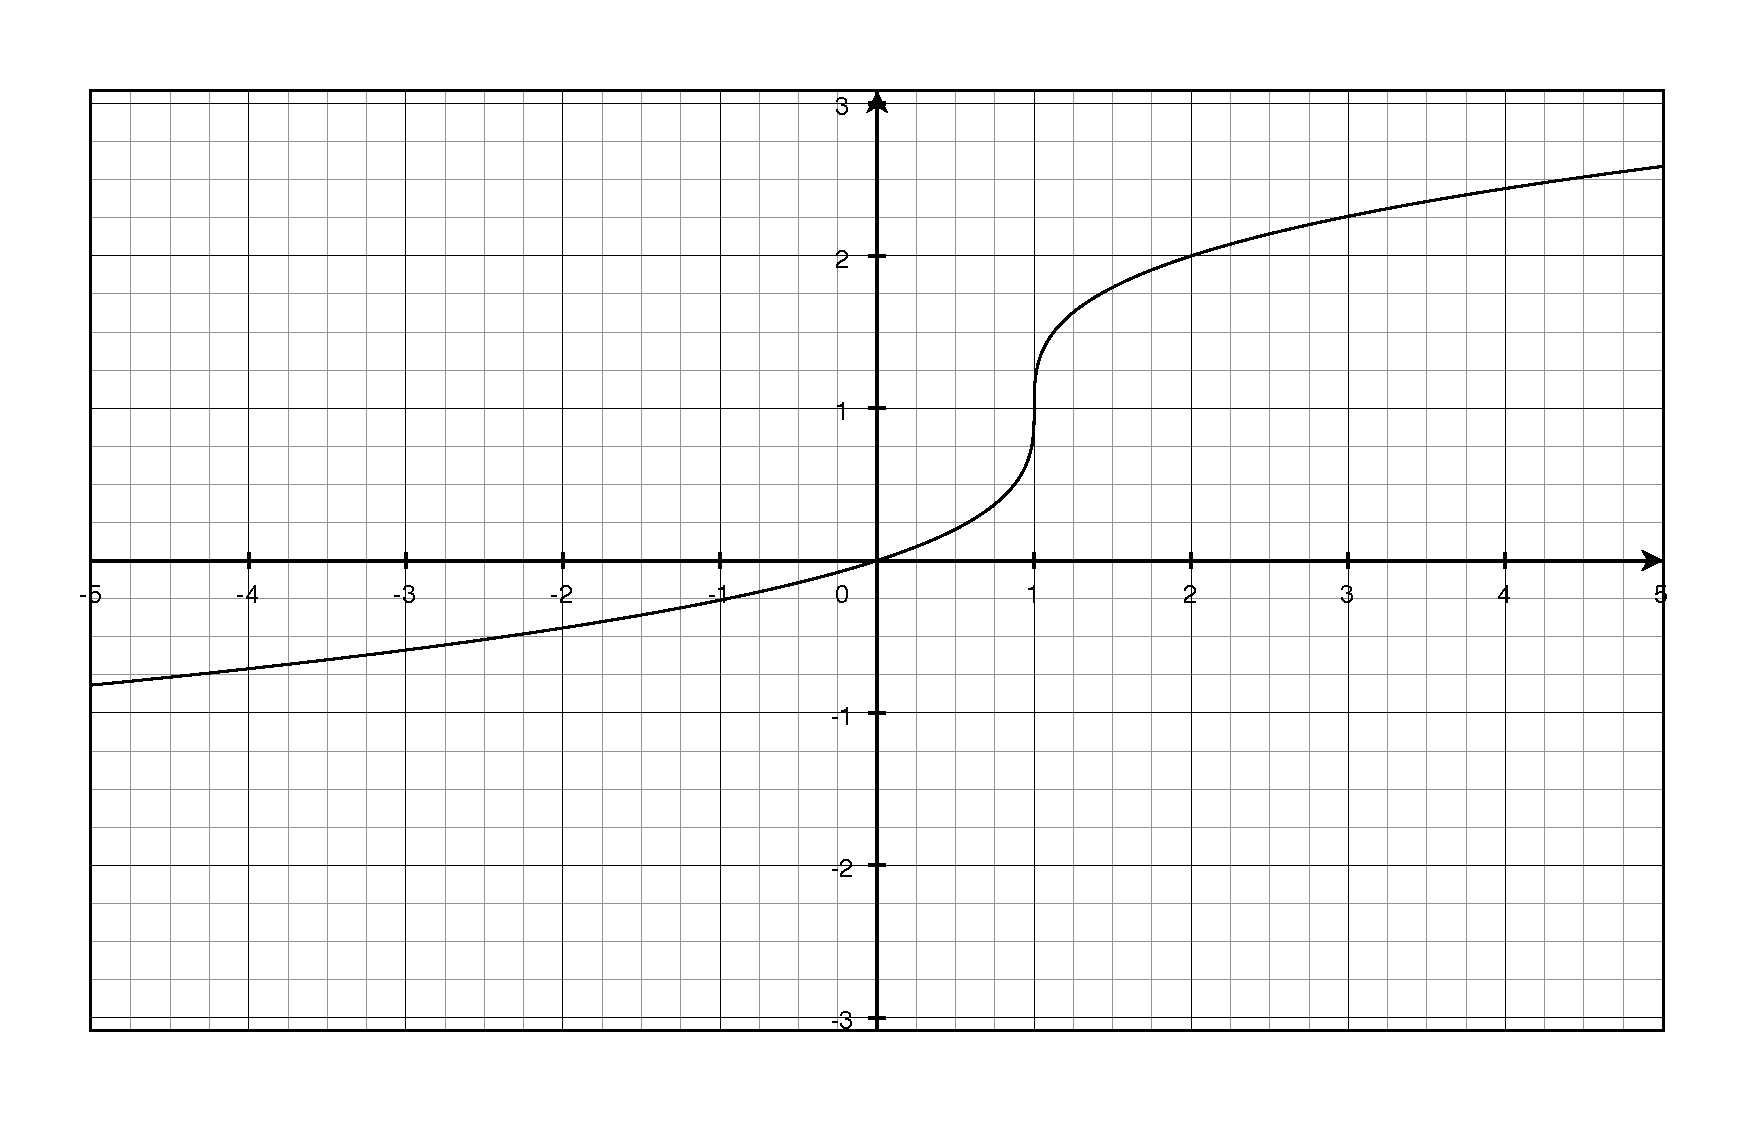
\includegraphics[scale=.3]{question7.eps}
%   \caption*{question 7}
% \end{figure}

% \begin{tabular}{cc}
%   \toprule
%   period & amplitude \\
%     $\pi$ & $2$ \\
%   \bottomrule
% \end{tabular}

\printanswers
\excludecomment{comment}

\ifprintanswers 
  \usepackage{2in1, lscape} 
\fi

\author{}
\date{\today}
\title{Math 142 \\ Homework Four}

\begin{document}

  \maketitle

  \section{Homework}
  Section 5.4: 

  \section{Extra Credit}
  TO DO

  \ifprintanswers

    \pagebreak

    \section{Section 5.4}
    \begin{description}

      \item[7]
        
        \begin{figure}[H]
          \centering
          \includegraphics[scale=0.9]{exercise07.eps}
          \caption{$f(x) = 4 \tan x$; period: $\pi$}
        \end{figure}

      \item[8]
        \begin{figure}[H]
          \centering
          \includegraphics[scale=0.9]{exercise08.eps}
          \caption{$f(x) = -4 \tan x$}; period: $\pi$
        \end{figure}

      \item[11]
        \begin{figure}[H]
          \centering
          \includegraphics[scale=0.9]{exercise11.eps}
          \caption{$f(x) = - \cot x$; period: $\pi$}
        \end{figure}

      \item[12]
        \begin{figure}[H]
          \centering
          \includegraphics[scale=0.9]{exercise12.eps}
          \caption{$f(x) = 2 \cot x$}; period: $\pi$
        \end{figure}

      \item[13]
        \begin{figure}[H]
          \centering
          \includegraphics[scale=0.9]{exercise13.eps}
          \caption{$f(x) = 2 \csc x$; period: $2 \pi$}
        \end{figure}

      \item[14]
        \begin{figure}[H]
          \centering
          \includegraphics[scale=0.9]{exercise14.eps}
          \caption{$f(x) = \frac{1}{2} \csc x$}; period: $2 \pi$
        \end{figure}

      \item[15]
        \begin{figure}[H]
          \centering
          \includegraphics[scale=0.9]{exercise15.eps}
          \caption{$f(x) = 3 \sec x$; period: $2 \pi$}
        \end{figure}

      \item[16]
        \begin{figure}[H]
          \centering
          \includegraphics[scale=0.9]{exercise16.eps}
          \caption{$f(x) = -3 \sec x$; period: $2 \pi$}
        \end{figure}

      \item[17]
        \begin{figure}[H]
          \centering
          \includegraphics[scale=0.9]{exercise17.eps}
          \caption{$f(x) = \tan \left( x + \frac{\pi}{2} \right)$; period: $\pi$}
        \end{figure}

      \item[18]
        \begin{figure}[H]
          \centering
          \includegraphics[scale=0.9]{exercise18.eps}
          \caption{$f(x) = \tan \left( x - \frac{\pi}{4} \right)$; period: $\pi$}
        \end{figure}

      \item[19]
        \begin{figure}[H]
          \centering
          \includegraphics[scale=0.9]{exercise19.eps}
          \caption{$f(x) = \csc \left( x - \frac{\pi}{2} \right)$; period: $2 \pi$}
        \end{figure}

      \item[20]
        \begin{figure}[H]
          \centering
          \includegraphics[scale=0.9]{exercise20.eps}
          \caption{$f(x) = \sec \left( x + \frac{\pi}{4} \right)$; period: $2 \pi$}
        \end{figure}

      \item[25]
        \begin{figure}[H]
          \centering
          \includegraphics[scale=0.9]{exercise25.eps}
          \caption{$f(x) = \tan 2x$; period: $\frac{\pi}{2}$}
        \end{figure}

      \item[26]
        \begin{figure}[H]
          \centering
          \includegraphics[scale=0.9]{exercise26.eps}
          \caption{$f(x) = \tan \frac{1}{2} x $; period: $2 \pi$}
        \end{figure}

      \item[27]
        \begin{figure}[H]
          \centering
          \includegraphics[scale=0.9]{exercise27.eps}
          \caption{$f(x) = \tan \frac{\pi}{4} x $; period: $4$}
        \end{figure}

      \item[28]
        \begin{figure}[H]
          \centering
          \includegraphics[scale=0.9]{exercise28.eps}
          \caption{$f(x) = \cot \frac{\pi}{2} x $; period: $2$}
        \end{figure}

      \item[29]
        \begin{figure}[H]
          \centering
          \includegraphics[scale=0.9]{exercise29.eps}
          \caption{$f(x) = \sec 2x $; period: $\pi$}
        \end{figure}

      \item[30]
        \begin{figure}[H]
          \centering
          \includegraphics[scale=0.9]{exercise30.eps}
          \caption{$f(x) = 5 \csc 3x $; period: ${2 \pi}{3}$}
        \end{figure}





    \end{description}
  \else
    \vspace{1 cm}
    \begin{quote}
      \begin{em}
        TO DO
      \end{em}
    \end{quote}
    \hspace{1 cm} --Shunryu Suzuki
  \fi

\end{document}

